%
% Modified by Megan Patnott
% Last Change: Jan 18, 2013
%
%%%%%%%%%%%%%%%%%%%%%%%%%%%%%%%%%%%%%%%%%%%%%%%%%%%%%%%%%%%%%%%%%%%%%%%%
%
% Modified by Sameer Vijay
% Last Change: Tue Jul 26 2005 13:00 CEST
%
%%%%%%%%%%%%%%%%%%%%%%%%%%%%%%%%%%%%%%%%%%%%%%%%%%%%%%%%%%%%%%%%%%%%%%%%
%
% Sample Notre Dame Thesis/Dissertation
% Using Donald Peterson's ndthesis classfile
%
% Written by Jeff Squyres and Don Peterson
%
% Provided by the Information Technology Committee of
%   the Graduate Student Union
%   http://www.gsu.nd.edu/
%
% Nothing in this document is serious except the format.  :-)
%
% If you have any suggestions, comments, questions, please send e-mail
% to: ndthesis@gsu.nd.edu
%
%%%%%%%%%%%%%%%%%%%%%%%%%%%%%%%%%%%%%%%%%%%%%%%%%%%%%%%%%%%%%%%%%%%%%%%%


%
% Chapter 5
%


\chapter{R-matrix analysis}
\label{chap: r-matrix}

An $R$-matrix analysis was performed to analyze the effects of the new lifetime and cross sections measurements described earlier. Such an analysis can be used to transform the cross sections into $S$-factors, which removes the Coulomb repulsion component of the cross-section and provides higher fidelity extrapolations to astrophysical energies. The $^{14}$N$(p,\gamma)^{15}$O system is ideal for $R$-matrix analysis because it is comprised of light nuclei with a discrete level structure at relatively low energies. While there are many programs available for performing $R$-matrix fits, we use the \texttt{AZURE2} code \cite{Azuma2010}, which was also used for similar, previous measurements \cite{Li2016}. 

\section{Impact of new lifetimes}
\label{sec: lifetime fit}

Following the analysis of \citet{Li2016}, the width of the 6.79 MeV state in $^{15}$O  was previously the largest source of uncertainty in the low-energy extrapolations of the cross section. A set of $R$-matrix fits was employed to explore the impact of our newly measured lifetimes. To isolate the effects of our measurement, we selected discrete lifetimes within our uncertainty range for the lifetime of the 6.79 MeV state in $^{15}$O, converted them to their equivalent radiative width, and used those level width values throughout the fit and extrapolation. This collection of fits, therefore, serves primarily as an illustration of the ways in which these new lifetime measurements impact the low energy extrapolations of the cross section.

In the fits presented here, the information about the levels was taken from  \citet{Ajzenberg-Selove1991} or \citet{Daigle2016} where updated. A channel radius of 5.5 fm was adopted for this work, which matches the analyses done by Refs.~\cite{Adelberger2011, Li2016, Wagner2018}. Information about the levels and their parameters as used in \texttt{AZURE2} are contained in Table~\ref{table: fitParams}. 


\begin{table*}[]
\thisfloatpagestyle{plain}
\caption{PARAMETERS USED IN THE $R$-MATRIX FITS FOR EXPLORING THE IMPACT OF NEWLY MEASURED LIFETIMES}
\begin{center}
\begin{threeparttable}
\begin{tabular}{c  c  c  c  c  c  c}
\toprule
$E_x$ (Ref.~\cite{Ajzenberg-Selove1991}) &   $E_x$ (fit) & $J^\pi$ & Channel & l & s & ANC (fm$^{-1/2}$) / $\Gamma$ (eV)\\ 
\midrule
0.0 & 0.0	& 1/2$^-$ &	$^{14}$N+p &	1&	1/2&	{0.23}\\
	&	&	    &    $^{14}$N+p &	1&	3/2&	{7.4} \\
%5.183(1) & \textbf{5.183}&	1/2$^+$&	$^{14}$N+p&	0&	1/2&	\textbf{0.33}\\
%	&	&		    &$^{15}$O+$\gamma_{0.00}$  &	E1&	1/2&	\textbf{0.0784}\\
%5.2409(3) & \textbf{5.2409}&	5/2$^+$&	$^{14}$N+p &	2&	1/2&	\textbf{0.23}\\
%                &	&		  & $^{14}$N+p &	2&	3/2&	\textbf{0.24}\\
%	 			&	&	 &$^{15}$O+$\gamma_{0.00}$	&M2&	1/2&	\textbf{0.0002}\\
%6.1763(17) & \textbf{6.1763}&	3/2$^-$& $^{14}$N+p &	1&	1/2&	\textbf{0.47}\\
%				&	&	& $^{14}$N+p	&1	&3/2	&\textbf{0.53}\\
%				&	&	&$^{15}$O+$\gamma_{0.00}$	&M1	&1/2&	\textbf{0.865}\\
6.7931(17) & {6.7931}&	3/2$^+$ & $^{14}$N+p &	0&	3/2&	{4.75}\\
	&	&	     &  $^{15}$O+$\gamma_{0.00}$	&  E1  &	1/2&	\textbf{2.50$^{\text{a}}$}\\
%	& &       &  $^{15}$O+$\gamma_{6.17}$	&  E1  &	3/2&{-0.002}\\
%6.8594(9) & \textbf{6.8594}&	5/2$^+$&	$^{14}$N+p&	2&	1/2&\textbf{0.39}\\
%	&		&    &     $^{14}$N+p&	2&	3/2&	\textbf{0.42}\\
%	&		&    &     $^{15}$O+$\gamma_{5.24}$&	M1&	5/2&	\textbf{0.04}\\
%7.2759(6) & \textbf{7.2759}&	7/2$^+$&	$^{14}$N+p &	2&	3/2&	\textbf{1541}\\
%	&		&    &     $^{15}$O+$\gamma_{5.24}$&	M1&	5/2&	\textbf{0.00099}\\
\hline
%7.5565(4) & 7.5563	&	1/2$^+$	&	$^{14}$N+p	&	0	&	1/2	&	\textbf{1.0$\times$10$^3$}	\\
%	&	&	&	$^{15}$O+$\gamma_{0.00}$	&	E1	&	1/2	&	\textbf{0.61$\times$10$^{-3}$}\\
%	&	&	&	$^{15}$O+$\gamma_{6.79}$	&	M1	&	3/2	&	\textbf{8.22$\times$10$^{-3}$}\\
%	&	&	&	$^{15}$O+$\gamma_{5.18}$	&	M1	&	1/2	&	\textbf{0.006}\\
%	&	&	&	$^{15}$O+$\gamma_{6.17}$	&	E1	&	3/2	&	\textbf{0.0254}\\
8.2840(5)& \textbf{8.2848}&	3/2$^+$	&	$^{14}$N+p	&	2	&	1/2	&	{-92.2}\\
	&	&	&	$^{14}$N+p	&	0	&	3/2	&	\textbf{4.013$\times$10$^3$}\\
	&	&	&	$^{14}$N+p	&	2	&	3/2	&	{-509}\\
	&	&	&	$^{15}$O+$\gamma_{0.00}$	&	E1	&	1/2	&	\textbf{0.244}\\
%	&	&	&	$^{15}$O+$\gamma_{5.18}$	&	M1	&	1/2	&	{0.01}\\
%	&	&	&	$^{15}$O+$\gamma_{5.24}$	&	M1	&	5/2	&	{0.2}\\
%	&	&	&	$^{15}$O+$\gamma_{6.17}$	&	E1	&	3/2	&	{-4$\times$10$^{-3}$}\\
%	&	&	&	$^{15}$O+$\gamma_{6.86}$	&	M1	&	5/2	&	{0.01}\\
%8.743(6) & \textbf{8.7502}&	1/2$^+$	&	$^{14}$N+p	&	0	&	1/2	&	\textbf{35.726$\times$10$^3$}\\
%	&	&	&	$^{15}$O+$\gamma_{5.18}$	&	M1	&	1/2	&	\textbf{-0.2}\\
%	&	&	&	$^{15}$O+$\gamma_{6.17}$	&	E1	&	3/2	&	\textbf{0.0827}\\
%8.922(2) & \textbf{8.9219}&	5/2$^+$	&	$^{14}$N+p	&	2	&	3/2	&	\textbf{3.8$\times$10$^3$}\\
%	&	&	&	$^{15}$O+$\gamma_{6.79}$	&	M1	&	3/2	&	\textbf{0.003}\\
8.9821(17) & {8.98}&	5/2$^-$	&	$^{14}$N+p	&	1	&	3/2	&	\textbf{-5.872$\times$10$^3$}\\
	&	&	&	$^{15}$O+$\gamma_{0.00}$	&	E2	&	1/2	&	\textbf{-0.303}\\
	&	&	&	$^{15}$O+$\gamma_{6.79}$	&	E1	&	3/2	&	{-0.001}\\
9.484(8) & \textbf{9.488}&	3/2$^+$	&	$^{14}$N+p	&	2	&	1/2	&	{77.69$\times$10$^3$}	\\
	&	&	&	$^{14}$N+p	&	0	&	3/2	&	\textbf{126.685$\times$10$^3$}	\\
	&	&	&	$^{14}$N+p	&	2	&	3/2	&	{-7.822$\times$10$^3$}\\
	&	&	&	$^{15}$O+$\gamma_{0.00}$	&	E1	&	1/2	&	\textbf{6.92}\\
%	&	&	&	$^{15}$O+$\gamma_{6.86}$	&	M1	&	5/2	&	{0.2}\\
9.488(3) & {9.4905}&	5/2$^-$	&	$^{14}$N+p	&	3	&	1/2	&	{0.979$\times$10$^3$}\\
	&	&	&	$^{14}$N+p	&	1	&	3/2	&	{-6.576$\times$10$^3$}\\
	&	&	&	$^{14}$N+p	&	3	&	3/2	&	{-0.985$\times$10$^3$}\\
	&	&	&	$^{15}$O+$\gamma_{0.00}$	&	E2	&	1/2	&	\textbf{-0.307}\\
	&	&	&	$^{15}$O+$\gamma_{6.79}$	&	E1	&	3/2	&	{-0.0123}\\
9.609(2) & {9.6075}&	3/2$^-$	&	$^{14}$N+p	&	1	&	3/2	&	\textbf{-13.821$\times$10$^3$}\\
	&	&	&	$^{15}$O+$\gamma_{0.00}$	&	M1	&	1/2	&	\textbf{1.24}\\
     &	&	&	$^{15}$O+$\gamma_{6.79}$	&	E1	&	3/2	&	{-0.044}\\
%	&	&	&	$^{15}$O+$\gamma_{5.24}$	&	E1	&	5/2	&	{0.095}\\
%10.2817 & \textbf{10.2817}	&	5/2$^+$	&	$^{14}$N+p	&	2	&	3/2	&	\textbf{17.292$\times$10$^3$}\\
%	&	&	&	$^{15}$O+$\gamma_{6.79}$	&	M1	&	3/2	&	\textbf{0.2}\\	
%	&	&	&	$^{15}$O+$\gamma_{6.86}$	&	M1	&	5/2	&	\textbf{-0.4}\\	
%10.480 & \textbf{10.4675}	&	3/2$^-$	&	$^{14}$N+p	&	1	&	1/2	&	\textbf{28.998$\times$10$^3$}\\
%	&	&	&	$^{14}$N+p	&	1	&	3/2	&	\textbf{9.652$\times$10$^3$}\\
%	&	&	&	$^{15}$O+$\gamma_{0.00}$	&	M1	&	1/2	&	\textbf{-0.404}\\	
%	&	&	&	$^{15}$O+$\gamma_{6.79}$	&	E1	&	3/2	&	\textbf{0.1}\\
%	&	&	&	$^{15}$O+$\gamma_{6.86}$	&	E1	&	5/2	&	\textbf{0.1}\\
%10.506 & \textbf{10.5313}&	3/2$^+$	&	$^{14}$N+p	&	0	&	3/2	&	\textbf{205$\times$10$^3$}\\
%	&	&	&	$^{15}$O+$\gamma_{0.00}$	&	E1	&	1/2	&	\textbf{-0.195}\\
%	&	&	&	$^{15}$O+$\gamma_{6.79}$	&	M1	&	3/2	&	\textbf{0.3}\\
%	&	&	&	$^{15}$O+$\gamma_{6.86}$	&	M1	&	5/2	&	\textbf{-0.4}\\
%10.9288 & \textbf{10.9288}&	7/2$^+$	&	$^{14}$N+p	&	2	&	3/2	&	\textbf{56.948$\times$10$^3$}\\
%	&	&	&	$^{15}$O+$\gamma_{6.79}$	&	E2&	3/2	&	\textbf{1}\\
%11.218(3) & 11.217(2)& 3/2$^+$&	$^{14}$N+p	&	0	&	3/2	&	\textbf{40$\times$10$^3$}\\
%	&	&	&	$^{15}$O+$\gamma_{0.00}$	&	E1	&	1/2	& 5.21	\\   	
& {15}	&	3/2$^+$	&	$^{14}$N+p	&	0	&	3/2	&	\textbf{4.722$\times$10$^6$}\\
	&	&	&	$^{15}$O+$\gamma_{0.00}$	&	E1	&	1/2	&	\textbf{327.3}	\\
%& \textbf{15}	&	5/2$^+$	&	$^{14}$N+p	&	2	&	1/2	&	\textbf{1.452$\times$10$^7$}\\
\bottomrule
\end{tabular}
\begin{tablenotes}
\small 
\item Levels used in the \textit{R}-matrix fits. Bold values indicate parameters which were allowed to vary during the fit. The signs on the partial widths and ANCs indicates the relative interferences. The dividing line demarcates the proton separation energy at $E_x$ = 7.2968(5) MeV \cite{Ajzenberg-Selove1991}. Levels where all parameters are fixed are not shown in this table for brevity but were included in the fits. a) Indicates the partial width of the 6.79 MeV state, measured in this experiment to between $\Gamma$ = 0.66 - 3.29 eV. For each individual fit, this width was fixed. However, between each fit, this width was varied to different values within our range to explore how the uncertainty in this measurement affects the low energy extrapolation. These different fits are shown in Fig.\ \ref{fig: rmatrixRange} and are otherwise identical.
\end{tablenotes}
\end{threeparttable}
\label{table: fitParams}
\end{center}
\end{table*}  



The cross-section data utilized in the fitting routine were from measurements at LUNA \cite{Formicola2004, Imbriani2005, Marta2008, Marta2011}, TUNL \cite{Runkle2005}, Bochum \cite{Schroder1987}, and the University of Notre Dame \cite{Li2016}. All of these data sets were left without scaling during the fits. The Bochum data from \citet{Schroder1987} were corrected as detailed in SFII \cite{Adelberger2011}. Additionally, the data used from \citet{Li2016} are a differential cross section taken at 45$\degree$ and are treated as such in the fits. This dataset was scaled by a factor of 4$\pi$ in the plotting only to compare to the angle integrated data. 



\begin{figure}[h!]
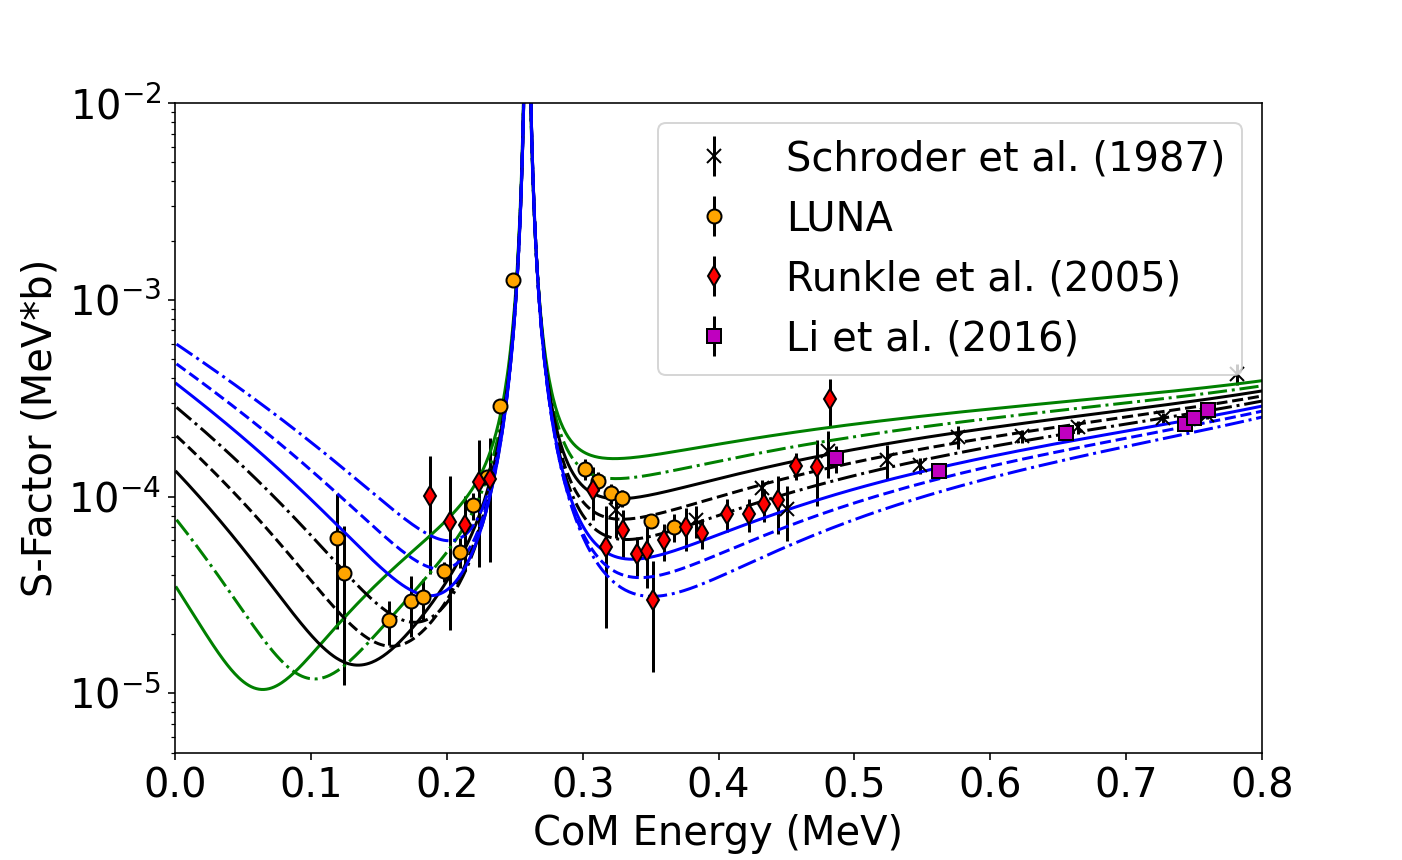
\includegraphics[width=1.0\linewidth]{./figures/lifetimeEffects.png}
\caption{$R$-Matrix fits exploring the uncertainty of our lifetime measurements to the low energy extrapolation. The width of the 6.79 MeV excited state in $^{15}$O is fixed during each fit and changed in each subsequent iteration to another value within our uncertainty range. This clearly shows that even though our lifetime result provides the most stringent limitation on the lifetime of this state, it still has an outsized effect on the low energy behavior of this reaction. The Schr{\"{o}}der et al.~data are from \cite{Schroder1987}, while the LUNA data represents the measurements \cite{Formicola2004, Imbriani2005, Marta2008, Marta2011}, the Runkle et al.~data are from \cite{Runkle2005}, and the Li et al.~data are from \cite{Li2016}. Of these, the data used from \citet{Li2016} are differential and were treated as such in the fitting but scaled up by 4$\pi$ for plotting purposes.}
\label{fig: rmatrixRange}
\end{figure}


\begin{figure}[h!]
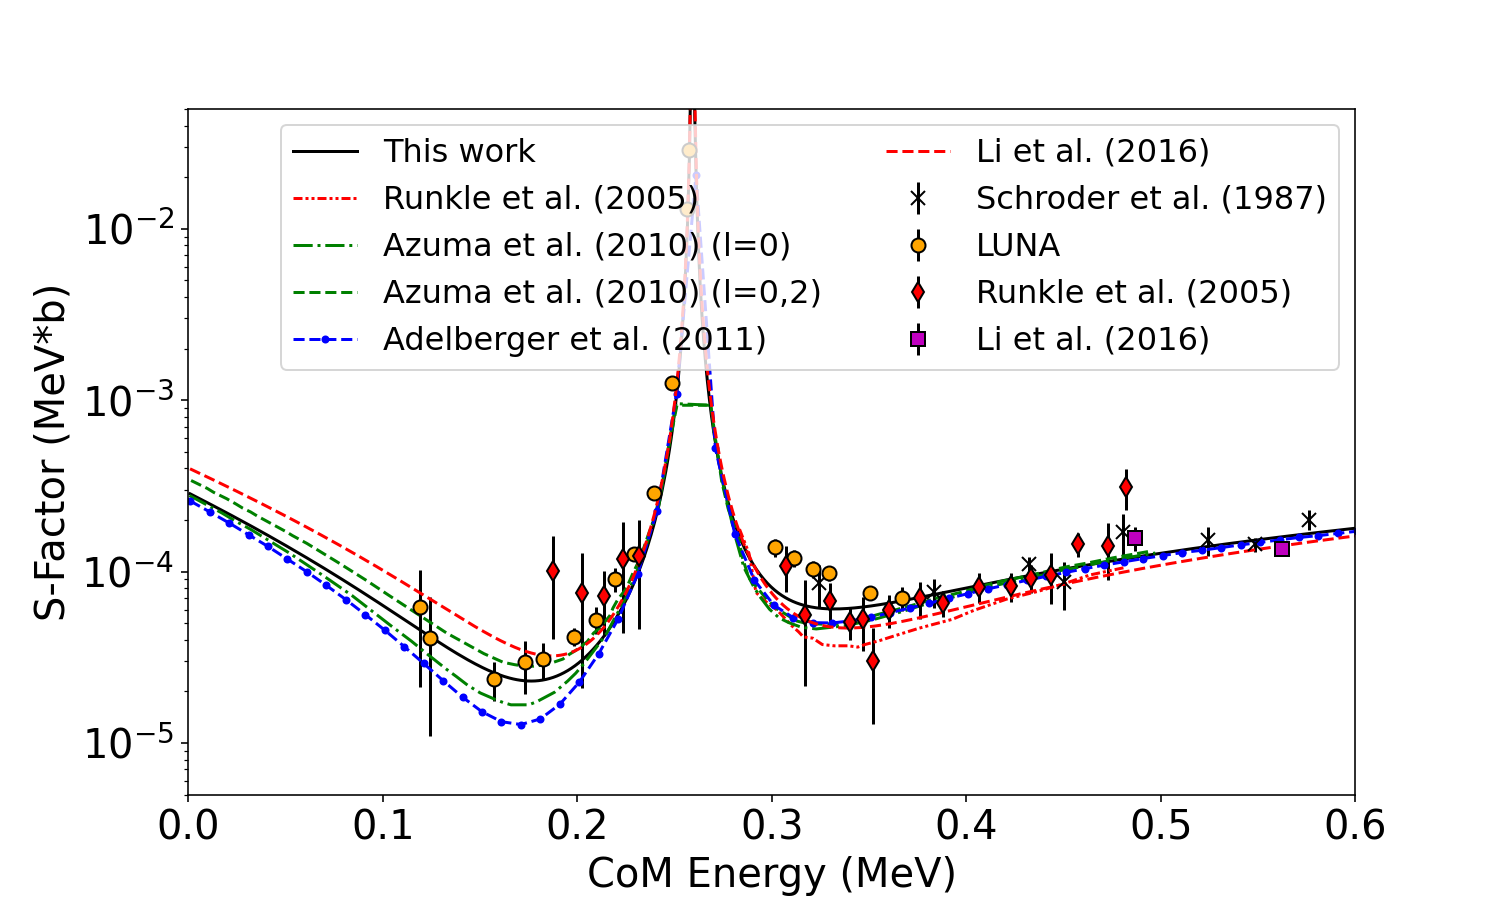
\includegraphics[width=1.0\linewidth]{./figures/bestFits.png}
\caption{$R$-matrix fits comparing our best fit with the lifetimes to those performed in previous works. Our fit used a lifetime value for the 6.79 MeV excited state in $^{15}$O within our measured range range, $\Gamma=2.75$ where the fits to the data provide good agreement with data above and below the 278 keV resonance. This plot is limited to the low energy region. The Schr{\"{o}}der et al.~data are from \cite{Schroder1987}, while the LUNA data represents the measurements of \cite{Formicola2004, Imbriani2005, Marta2008, Marta2011}, the Runkle et al.~data are from \cite{Runkle2005}, and the Li et al.~data are from \cite{Li2016}. Of these, the data used from \citet{Li2016} are differential and were treated as such in the fitting but scaled up by 4$\pi$ for plotting purposes. The fits from previous works come from Refs.~\cite{Runkle2005, Azuma2010, Adelberger2011, Li2016}.}
\label{fig: rmatrixClose}
\end{figure}

In examining the capture to the ground state in $^{15}$O, the $R$-matrix fits show the effect of our lifetime measurement. Specifically, in Fig.~\ref{fig: rmatrixRange}, we present fits showing the whole range of lifetimes for the 6.79 MeV state of $\tau = 0.6 \pm 0.4$. This shows that despite this measurement providing the most stringent limit on the lifetime, this range still translates into dramatic changes in the low energy behavior of the $S$-factor. Our fits, however, agree well with the capture data and previous studies. One of the best fits using our lifetimes is shown alongside fits from Refs.~\cite{Runkle2005, Azuma2010, Adelberger2011, Li2016} in Fig.~\ref{fig: rmatrixClose}. 

While the experimental results limit the previous uncertainty range in the lifetime data, this $R$-matrix analysis clearly demonstrates that it remains too large for solely reducing uncertainty in the extrapolation for the low energy range cross section of the ground state transition.

\section{Complete fit}
\label{sec: complete fit}


Since our new lifetime measurements still do not significantly limit the extrapolated uncertainty of the low-energy cross section, an $R$-matrix analysis was used to fit all the ground state and the 6.79 MeV transition differential cross section data measured in the current experiment, incorporating the new lifetimes, and an exhaustive set of previously measured data, which includes both cross section data and elastic scattering data. This, then, provides significantly greater constraint than the lifetime alone and ensures the most robust fit and extrapolation for the low-energy behavior of the $^{14}$N$(p,\gamma)^{15}$O reaction.

Similar to the fits for examining the lifetime's effects, the information about the levels was obtained from  \citet{Ajzenberg-Selove1991} or \citet{Daigle2016} where they had been updated. A channel radius of 5.5 fm was adopted for the fits, which matches the analyses done by Refs.~\cite{Adelberger2011, Li2016, Wagner2018}. Information about the levels and their parameters as used in \texttt{AZURE2} are contained in Table~\ref{table: fitParamsFullFit}. 


\begin{table*}[]
\thisfloatpagestyle{plain}
\caption{PARAMETERS USED IN THE COMPLETE $R$-MATRIX FIT}
\begin{center}
\begin{threeparttable}
\begin{tabular}{c  c  c  c  c  c  c}
\toprule
$E_x$ (Ref.~\cite{Ajzenberg-Selove1991}) &   $E_x$ (fit) & $J^\pi$ & Channel & l & s & ANC (fm$^{-1/2}$) / $\Gamma$ (eV)\\ 
\midrule
0.0 & 0.0	& 1/2$^-$ &	$^{14}$N+p &	1&	1/2&	{0.23}\\
	&	&	    &    $^{14}$N+p &	1&	3/2&	{7.4} \\
%5.183(1) & \textbf{5.183}&	1/2$^+$&	$^{14}$N+p&	0&	1/2&	\textbf{0.33}\\
%	&	&		    &$^{15}$O+$\gamma_{0.00}$  &	E1&	1/2&	\textbf{0.0784}\\
%5.2409(3) & \textbf{5.2409}&	5/2$^+$&	$^{14}$N+p &	2&	1/2&	\textbf{0.23}\\
%                &	&		  & $^{14}$N+p &	2&	3/2&	\textbf{0.24}\\
%	 			&	&	 &$^{15}$O+$\gamma_{0.00}$	&M2&	1/2&	\textbf{0.0002}\\
%6.1763(17) & \textbf{6.1763}&	3/2$^-$& $^{14}$N+p &	1&	1/2&	\textbf{0.47}\\
%				&	&	& $^{14}$N+p	&1	&3/2	&\textbf{0.53}\\
%				&	&	&$^{15}$O+$\gamma_{0.00}$	&M1	&1/2&	\textbf{0.865}\\
6.7931(17) & {6.7931}&	3/2$^+$ & $^{14}$N+p &	0&	3/2&	{4.75}\\
	&	&	     &  $^{15}$O+$\gamma_{0.00}$	&  E1  &	1/2&	\textbf{2.50$^{\text{a}}$}\\
%	& &       &  $^{15}$O+$\gamma_{6.17}$	&  E1  &	3/2&{-0.002}\\
%6.8594(9) & \textbf{6.8594}&	5/2$^+$&	$^{14}$N+p&	2&	1/2&\textbf{0.39}\\
%	&		&    &     $^{14}$N+p&	2&	3/2&	\textbf{0.42}\\
%	&		&    &     $^{15}$O+$\gamma_{5.24}$&	M1&	5/2&	\textbf{0.04}\\
%7.2759(6) & \textbf{7.2759}&	7/2$^+$&	$^{14}$N+p &	2&	3/2&	\textbf{1541}\\
%	&		&    &     $^{15}$O+$\gamma_{5.24}$&	M1&	5/2&	\textbf{0.00099}\\
\hline
%7.5565(4) & 7.5563	&	1/2$^+$	&	$^{14}$N+p	&	0	&	1/2	&	\textbf{1.0$\times$10$^3$}	\\
%	&	&	&	$^{15}$O+$\gamma_{0.00}$	&	E1	&	1/2	&	\textbf{0.61$\times$10$^{-3}$}\\
%	&	&	&	$^{15}$O+$\gamma_{6.79}$	&	M1	&	3/2	&	\textbf{8.22$\times$10$^{-3}$}\\
%	&	&	&	$^{15}$O+$\gamma_{5.18}$	&	M1	&	1/2	&	\textbf{0.006}\\
%	&	&	&	$^{15}$O+$\gamma_{6.17}$	&	E1	&	3/2	&	\textbf{0.0254}\\
8.2840(5)& \textbf{8.2848}&	3/2$^+$	&	$^{14}$N+p	&	2	&	1/2	&	{-92.2}\\
	&	&	&	$^{14}$N+p	&	0	&	3/2	&	\textbf{4.013$\times$10$^3$}\\
	&	&	&	$^{14}$N+p	&	2	&	3/2	&	{-509}\\
	&	&	&	$^{15}$O+$\gamma_{0.00}$	&	E1	&	1/2	&	\textbf{0.244}\\
%	&	&	&	$^{15}$O+$\gamma_{5.18}$	&	M1	&	1/2	&	{0.01}\\
%	&	&	&	$^{15}$O+$\gamma_{5.24}$	&	M1	&	5/2	&	{0.2}\\
%	&	&	&	$^{15}$O+$\gamma_{6.17}$	&	E1	&	3/2	&	{-4$\times$10$^{-3}$}\\
%	&	&	&	$^{15}$O+$\gamma_{6.86}$	&	M1	&	5/2	&	{0.01}\\
%8.743(6) & \textbf{8.7502}&	1/2$^+$	&	$^{14}$N+p	&	0	&	1/2	&	\textbf{35.726$\times$10$^3$}\\
%	&	&	&	$^{15}$O+$\gamma_{5.18}$	&	M1	&	1/2	&	\textbf{-0.2}\\
%	&	&	&	$^{15}$O+$\gamma_{6.17}$	&	E1	&	3/2	&	\textbf{0.0827}\\
%8.922(2) & \textbf{8.9219}&	5/2$^+$	&	$^{14}$N+p	&	2	&	3/2	&	\textbf{3.8$\times$10$^3$}\\
%	&	&	&	$^{15}$O+$\gamma_{6.79}$	&	M1	&	3/2	&	\textbf{0.003}\\
8.9821(17) & {8.98}&	5/2$^-$	&	$^{14}$N+p	&	1	&	3/2	&	\textbf{-5.872$\times$10$^3$}\\
	&	&	&	$^{15}$O+$\gamma_{0.00}$	&	E2	&	1/2	&	\textbf{-0.303}\\
	&	&	&	$^{15}$O+$\gamma_{6.79}$	&	E1	&	3/2	&	{-0.001}\\
9.484(8) & \textbf{9.488}&	3/2$^+$	&	$^{14}$N+p	&	2	&	1/2	&	{77.69$\times$10$^3$}	\\
	&	&	&	$^{14}$N+p	&	0	&	3/2	&	\textbf{126.685$\times$10$^3$}	\\
	&	&	&	$^{14}$N+p	&	2	&	3/2	&	{-7.822$\times$10$^3$}\\
	&	&	&	$^{15}$O+$\gamma_{0.00}$	&	E1	&	1/2	&	\textbf{6.92}\\
%	&	&	&	$^{15}$O+$\gamma_{6.86}$	&	M1	&	5/2	&	{0.2}\\
9.488(3) & {9.4905}&	5/2$^-$	&	$^{14}$N+p	&	3	&	1/2	&	{0.979$\times$10$^3$}\\
	&	&	&	$^{14}$N+p	&	1	&	3/2	&	{-6.576$\times$10$^3$}\\
	&	&	&	$^{14}$N+p	&	3	&	3/2	&	{-0.985$\times$10$^3$}\\
	&	&	&	$^{15}$O+$\gamma_{0.00}$	&	E2	&	1/2	&	\textbf{-0.307}\\
	&	&	&	$^{15}$O+$\gamma_{6.79}$	&	E1	&	3/2	&	{-0.0123}\\
9.609(2) & {9.6075}&	3/2$^-$	&	$^{14}$N+p	&	1	&	3/2	&	\textbf{-13.821$\times$10$^3$}\\
	&	&	&	$^{15}$O+$\gamma_{0.00}$	&	M1	&	1/2	&	\textbf{1.24}\\
     &	&	&	$^{15}$O+$\gamma_{6.79}$	&	E1	&	3/2	&	{-0.044}\\
%	&	&	&	$^{15}$O+$\gamma_{5.24}$	&	E1	&	5/2	&	{0.095}\\
%10.2817 & \textbf{10.2817}	&	5/2$^+$	&	$^{14}$N+p	&	2	&	3/2	&	\textbf{17.292$\times$10$^3$}\\
%	&	&	&	$^{15}$O+$\gamma_{6.79}$	&	M1	&	3/2	&	\textbf{0.2}\\	
%	&	&	&	$^{15}$O+$\gamma_{6.86}$	&	M1	&	5/2	&	\textbf{-0.4}\\	
%10.480 & \textbf{10.4675}	&	3/2$^-$	&	$^{14}$N+p	&	1	&	1/2	&	\textbf{28.998$\times$10$^3$}\\
%	&	&	&	$^{14}$N+p	&	1	&	3/2	&	\textbf{9.652$\times$10$^3$}\\
%	&	&	&	$^{15}$O+$\gamma_{0.00}$	&	M1	&	1/2	&	\textbf{-0.404}\\	
%	&	&	&	$^{15}$O+$\gamma_{6.79}$	&	E1	&	3/2	&	\textbf{0.1}\\
%	&	&	&	$^{15}$O+$\gamma_{6.86}$	&	E1	&	5/2	&	\textbf{0.1}\\
%10.506 & \textbf{10.5313}&	3/2$^+$	&	$^{14}$N+p	&	0	&	3/2	&	\textbf{205$\times$10$^3$}\\
%	&	&	&	$^{15}$O+$\gamma_{0.00}$	&	E1	&	1/2	&	\textbf{-0.195}\\
%	&	&	&	$^{15}$O+$\gamma_{6.79}$	&	M1	&	3/2	&	\textbf{0.3}\\
%	&	&	&	$^{15}$O+$\gamma_{6.86}$	&	M1	&	5/2	&	\textbf{-0.4}\\
%10.9288 & \textbf{10.9288}&	7/2$^+$	&	$^{14}$N+p	&	2	&	3/2	&	\textbf{56.948$\times$10$^3$}\\
%	&	&	&	$^{15}$O+$\gamma_{6.79}$	&	E2&	3/2	&	\textbf{1}\\
%11.218(3) & 11.217(2)& 3/2$^+$&	$^{14}$N+p	&	0	&	3/2	&	\textbf{40$\times$10$^3$}\\
%	&	&	&	$^{15}$O+$\gamma_{0.00}$	&	E1	&	1/2	& 5.21	\\   	
& {15}	&	3/2$^+$	&	$^{14}$N+p	&	0	&	3/2	&	\textbf{4.722$\times$10$^6$}\\
	&	&	&	$^{15}$O+$\gamma_{0.00}$	&	E1	&	1/2	&	\textbf{327.3}	\\
%& \textbf{15}	&	5/2$^+$	&	$^{14}$N+p	&	2	&	1/2	&	\textbf{1.452$\times$10$^7$}\\
\bottomrule
\end{tabular}
\begin{tablenotes}
\small 
\item Levels used in the complete \textit{R}-matrix fit to the whole set of data. Bold values indicate parameters which were allowed to vary during the fit. The signs on the partial widths and ANCs indicates the relative interferences. The dividing line demarcates the proton separation energy at $E_x$ = 7.2968(5) MeV \cite{Ajzenberg-Selove1991}. Levels where all parameters are fixed are not shown in this table for brevity but were included in the fits.
\item \textbf{THIS NEEDS TO BE CHANGED FOR THE NEW FITS WHEN THEY'VE BEEN COMPLETED}
\end{tablenotes}
\end{threeparttable}
\label{table: fitParams}
\end{center}
\end{table*}  



The cross-section data utilized in the fitting routine were from measurements at LUNA \cite{Formicola2004, Imbriani2005, Marta2008, Marta2011}, TUNL \cite{Runkle2005}, Bochum \cite{Schroder1987}, and the University of Notre Dame \cite{Li2016}. All of these data sets were left without scaling during the fits. The Bochum data from \citet{Schroder1987} were corrected as detailed in SFII \cite{Adelberger2011}. Additionally, the data used from \citet{Li2016} are a differential cross section taken at 45$\degree$ and are treated as such in the fits. This dataset was scaled by a factor of 4$\pi$ in the plotting only to compare to the angle integrated data. We chose to exclude the data from \citet{Wagner2018} in the fitting due to its large disagreement to other measurements. This data was, however, shown in plots alongside the other data to show their relation.

This elastic scattering data incorporated in this analysis were from....

\textbf{FROM HERE, ONCE THE SUMMING CORRECTIONS TO THE GROUND STATE HAVE BEEN COMPLETE I NEED TO FINISH THE FITS. THIS WILL THEN LET ME DISCUSS HOW THESE NEW DATA IMPACT THE FITS AND HOW THE EXTRAPOLATION TO LOW ENERGIES BEHAVES. I THINK THAT IS ALL THAT IS LEFT TO FINISH THIS SECTION.}

The extrapolations of the $S$-factors to zero energy for both measured transitions were calculated with the parameters from the \texttt{AZURE2} fit. From these, we recommend values of $S_{6.79}(0) = XXX$ keV b, which is very robust with all fits and agrees well with previous measurements. Furthermore, we recommend $S_{gs}(0) = XXX$ keV b which \textbf{RELATES TO OTHER MEASUREMENTS SOMEHOW}. 


% % uncomment the following lines,
% if using chapter-wise bibliography
%
% \bibliographystyle{ndnatbib}
% \bibliography{example}
